\chapter{Auxiliary projects} \label{app:auxiliary-projects}

This appendix describes three research efforts where I participated that are tangentially related to my work in semantic similarity. Although none of them contributed to the direct research and development in semantic similarity, they were useful in two senses:
\begin{paralist}
    \item they helped me be more familiar with the practices of knowledge representation, data federation and information sharing; and
    \item they provided a means for me to be acquainted with particular examples of contexts where application of semantic similarity is used as part of other, bigger systems.
\end{paralist}


\section{Semantic web in the Epidemic Marketplace}
\label{sec:auxiliary-projects/epiwork}

During the course of one year, I participated in the Epiwork project, an European project that ran from 2009 to~2013, funded by the Seventh Framework Program (FP7). This project aimed at developing the appropriate framework of tools and knowledge to design epidemic forecast infrastructures. The tasks assigned to the LaSIGE partner were:
\begin{itemize}
    \item to develop the Epidemic Marketplace (EM), a repository of epidemiological data;
    \item to create a website that serves as the front-end to the repository; and
    \item to define ways to annotate the repository data.
\end{itemize}

I participated in this project as an expert on semantic web. Namely, I was in charge of
\begin{paralist}
    \item making the data more accessible from the semantic web point of view, particularly to the other partners and their automatic tools, as well as
    \item increasing the digital preservation of the resources in the EM.
\end{paralist}
My participation has culminated in two contributions:
\begin{itemize}
    \item a semantic metadata model designed with the specific needs of epidemiology data in mind, which was used to guide the annotation process of the epidemiology resources~\citep{Couto2012}; and
    \item a Network of Epidemiology-Related Ontologies (NERO) representing most of the domains of epidemiology (chemistry concepts, diseases, symptoms, environmental conditions, methods of transmission, vaccines, sociology, geography, \etc.), to be used as source of concepts in the metadata of the resources~\citep{Ferreira2012}.
\end{itemize}

The metadata model defines a set of \emph{slots} that provide data owners specific topics relevant for epidemiological data, which can be used to guide the annotation process. It is based on the Dublin Core, a vocabulary of terms used to describe web resources (\eg video, images, web pages), as well as physical resources (\eg books, music records, artwork)~\citep{DCMI2012}. Being based on a popular standard for annotation is an advantage in three fronts:
\begin{enumerate}
    \item Most of the necessary information needed to describe a resource already exists (terms such as author, publication date, references, \etc.); we had to add only epidemiology-specific terms.
    \item It increases interoperability.
    \item It ensures long term usability, which contributes to the preservation of the data. In effect, while the EM website has been discontinued, due to the lack of funds, the data still exists, as well as their annotations.
\end{enumerate}

The metadata model is divided in three sections~\citep{Ferreira2013a}:
\begin{paralist}
    \item a technical section that contains terms related to the digital nature of the resources (their unique identifier, the name of the EM user that uploaded the data, the date of submission, \etc.);
    \item a general section, containing the non-epidemiology-related information of the resource (title, author, description, creation date, \etc.); and
    \item a content-specific section, with terms specific to epidemiology, including information on diseases, symptoms, social conditions, \etc.
\end{paralist}

Most of the content-specific metadata is meant to be provided by the user as ontology concept identifiers. Using ontologies to fill the metadata of a resource contributes to its machine-readability, but also to the preservation of the data. Ontologies provide:
\begin{itemize}
    \item an objective and traceable meaning to the metadata;
    \item a controlled vocabulary, thus contributing to the interoperability of the metadata with other semantic web systems;
    \item a language agnostic vocabulary, which avoids the pitfalls of natural language processing; and finally
    \item support for reasoning and other semantic tools (such as semantic similarity).
\end{itemize}

\begin{figure}
    \centering
    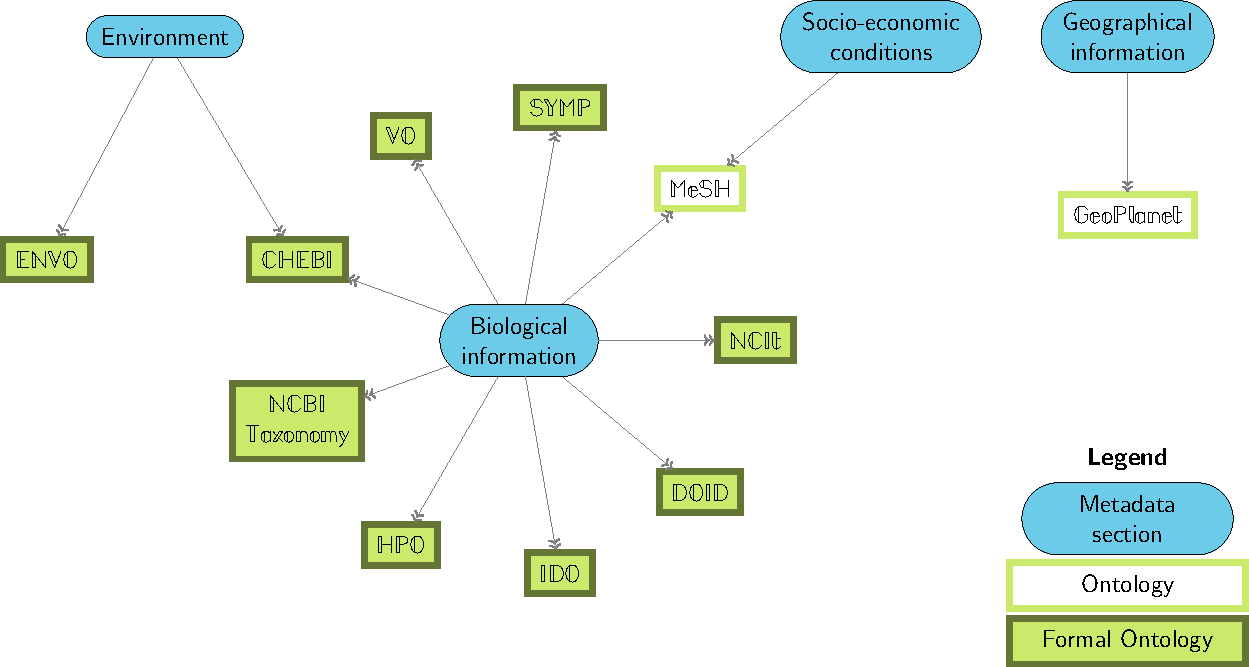
\includegraphics[width=0.9\textwidth]{images/nero.pdf}
    \caption[The Network of Epidemiology-Related Ontologies]{This figure represents NERO as a set of metadata sections (represented as blue round rectangles) and the ontologies used to annotate the epidemiology resources (in straight rectangles). Each metadata section is associated with a set of ontologies that contain the concepts relevant for that section. There is a difference between formal ontologies (represented with the shaded green background) and the other vocabularies, as explained in the last paragraph of \appref{app:ontologies}.}
    \label{fig:nero}
\end{figure}

To maximise the benefits of using ontologies, I contributed to the establishment of the Network of Epidemiology-Related Ontologies (NERO). This is a multi-domain collection of ontologies that represent parts of the epidemiology field: \eg diseases, symptoms, chemical compounds, modes of transmission, \etc. It also contain non-biomedical ontologies to represent demography, environmental conditions, geographical regions and socio-economic conditions. NERO was integrated in the Epidemic Marketplace as a way to facilitate annotation of resources, by suggesting concepts based on the content of the resource and facilitating the annotation process with an auto-complete-like feature that suggested concepts from those ontologies. As such, NERO bridges the gap between automatic systems and epidemiology, a domain which traditionally makes poor use of computer power (possibly because of its high heterogeneity), by bringing the semantic web into it. In fact, prior to NERO, there was not an expressive way to annotate resources with ontology concepts in this field. \figref{fig:nero} contains a graphical representation of which ontologies are used to fill the metadata model for an epidemiology resource.


\section{Text-mining} \label{sec:auxiliary-projects/text-mining}

Text-mining aims at extracting relevant information from unstructured natural text. The meaning of ``relevant'' depends on the actual goals of the text-mining process: for example, automatic news processing systems can perform ``Sentiment analysis'', a technique that detects whether the opinions expressed in text (in a full article, a blog post, a tweet, \etc.)\ is positive or negative; advanced algorithms can even classify text based on more specific emotional states, such as ``angry'', ``sad'' or ``happy''. In the biomedical domain, text mining is an important part of scientific discovery: it can be used to find drug targets and biomarkers, for drug repositioning, to create a clinical overview of a certain therapeutic area, to create domain specific databases, \etc.~\citep{Fleuren2015}.

The first preliminary study I was part of, in the context of text mining, was the application of semantic similarity to disambiguate geographical names in news articles~\citep{Batista2012}. Names of geographical features (called ``toponyms'') are particularly ambiguous: a particular case is in the name \emph{Lisboa}, which represents up to $41$~different locations in the territory of Portugal alone, from streets to a municipality, a city and a region. Being able to properly identify which place is being referred to in text is important to further process that text. One way to achieve this is by:
\begin{enumerate}
    \item associating each toponym with a set of its possible locations;
    \item comparing all the locations within each possible arrangement using semantic similarity;
    \item finding the arrangement with highest overall similarity score and choose it as the disambiguated set of locations.
\end{enumerate}

In this work, we used Geo-Net-PT, a geographical ontology of the Portuguese territory, which contains more than $400{,}000$ geographical locations, organised in a hierarchy (\eg \term{Portugal} \prop{contains} \term{Lisbon city}). This hierarchy can be used to compute semantic similarity with the algorithms mentioned in the main document, thus allowing the disambiguation process above.

I have also contributed to text-mining approaches in the biomedical domain. One of the most important tasks in text processing in biomedical informatics is the identification of entities such as chemical compounds in text. This allows further processing (for example, the detection of interaction between compounds). I have worked as a semantic similarity expert with a set of colleagues in text-mining in this context. In a first step, we investigated whether semantic similarity can be used to disambiguate chemical names in text, just like I had done previously in the geographical domain~\citep{Lamurias2015}. In a second step, we investigated whether semantic similarity can also be used to improve the overall performance a system designed to find interactions between two chemical compounds in text~\citep{Lamurias2014}. For example, the sentence ``\emph{Trilostane} may interact with \emph{aminoglutethimide}, causing too great a decrease in adrenal function'' describes the interaction between two compounds (in slanted text), which the system is able to find. Semantic similarity was used here in an effort to reduce false positive interactions found by the system.


\section{Ontology alignment} \label{sec:auxiliary-projects/alignment}

Part of my research in multiple-ontology semantic similarity was dedicated to the study of ontology alignment techniques. As explained throughout this document, multi-ontology semantic similarity is enhanced if the ontologies used to compute similarity are related to each other in some way. In general ontology alignment is done by asserting that two concepts from different ontologies are equivalent. In the context of multiple-ontology single-domain measures (see \secref{sec:sota/multi-ontology}), complementary ontologies improve the accuracy of similarity only if the ontologies are \emph{linked}.

\begin{figure}
    \centering
    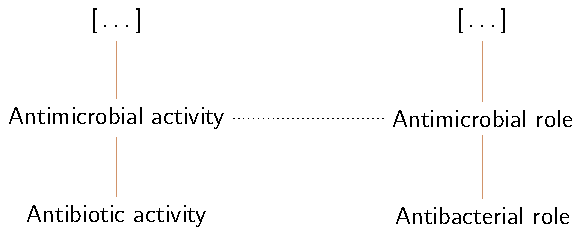
\includegraphics{images/alignment.pdf}
    \caption[Partial alignment between two ontologies of the biochemical domain]{The two ontologies partially illustrated here represent the same domain of reality, namely the roles of biochemical molecules. The dotted line represents an \emph{equivalence} link between the two, and can be explored by multiple-ontology semantic similarity to compare concepts in different ontologies.}
    \label{fig:simple-match}
\end{figure}

For example, with the aligned pair of ontologies in \figref{fig:simple-match}, it would be possible to assign a relatively high value to the similarity between \term{Antibiotic activity} and \term{Antibacterial role}, but only if their parent concepts (\term{Antimicrobial activity} and \term{Antimicrobial role} respectively) are explicitly marked as \emph{equivalent}, as the dotted line suggests.

The set of equivalences between multiple ontologies (called an \emph{alignment}) is, therefore, essential to single-domain multiple-ontology similarity measures. However, finding them is labour-intensive, given the amount of concepts in biomedical ontologies, which has lead the community to develop ``ontology matching'' algorithms, which find, automatically or semi-automatically, equivalent concepts within two or more ontologies~\citep{Euzenat2007}. Ontology alignments can be made with simple textual matching, which rely on dictionaries and thesauri to increase their recall (for instance, the fact that ``activity'' and ``role'' are synonyms might be used to match the two concepts in the ontologies from \figref{fig:simple-match}); they can also leverage on the structure of the ontologies to find related concepts (concepts with many linked subclasses should themselves be linked); and they can also explore the logical definitions on the ontologies to find these matches~\citep{Shvaiko2005}.

During the early stages of my PhD, I worked under the assumption that ontology alignment would be essential for my research. As such, I participated in Semantic Ontology Matching using External Resources (SOMER), a project funded by the Fundação para a Ciência e Tecnologia (the Portuguese Foundation for Science and Technology), and which ran from 2012 to~2014. One of the tasks that I developed was the alignment of geographical ontologies (namely the Yahoo!~GeoPlanet, a geography ontology for world-wide locations, and the Geo-Net-PT, mentioned above).

As it turns out, ontologies that represent different domains of the biomedical information are usually already quite orthogonal, given the OBO Foundry's principles and the best practices in ontology development (see \appref{app:ontologies}) and, therefore, this technique is not vital for the calculation of similarity among concepts from different ontologies. As such, the total effort that I put into this project, with regard to my PhD, was relatively small when compared to other endeavours, since I recognised that the outputs of the project would not benefit multi-domain semantic similarity to a large extent.

